\documentclass{article}
% Force natbib into numerical citation mode (NeurIPS expects numeric citations).
% IMPORTANT: this must appear before loading neurips_2023, which loads natbib internally.
\PassOptionsToPackage{numbers,sort&compress}{natbib}
\usepackage[final]{neurips_2023}
\usepackage{amsmath,amssymb}
\usepackage{tikz}
\usepackage{graphicx}
\usepackage{float}
\usepackage{booktabs}
\usepackage{hyperref}
\graphicspath{{figures/}}

\usetikzlibrary{arrows.meta,positioning}

% narrower margins (wider text block)
\AtBeginDocument{
  \newgeometry{
    textheight=9in,
    textwidth=7in,
    top=1in,
    headheight=12pt,
    headsep=25pt,
    footskip=30pt
  }
}

% remove NeurIPS footer on first page
\makeatletter
\renewcommand{\@notice}{}
\makeatother

\title{Transfer Learning: Exploring Two-Headed CNN w/Interaction Loss vs. Two separate
		CNN Models for
Superclass/Subclass Classification}

\author{
		Christian Montgomery and Aksel Kretsinger-Walters \\
		Columbia University \\
		\texttt{cm4521@columbia.edu, adk2164@columbia.edu}
}

\begin{document}

\maketitle
\vspace{-3em}

\section{Introduction}

We explored optimal techniques of transfer learning for the multi-label image
classification task, predicting
superclass (bird/dog/reptile/novel class) and subclasses (87 seen + novel subclass) for a
selection of $64
\times 64$ images. The main challenge to overcome was distribution shift between the
training and test
datasets, and novel classes appearing at test time (identifying both new superclasses and
new subclasses as ``novel'').

To maximize our performance on this classification, we explored two different model architectures: a
multi-headed CNN with KL Interaction term, and separately two distinct CNN's for each
classification task. We
trained detecting for ``novel'' superclasses via including some out-of-distribution data
from CIFAR 100, and
held-out some subclass images from training to assess pseudo-novel detection. For both
classifications, we
tuned a threshold on the max softmax score for each image, implying whether it
represented a novel class or
not. Two other areas we explored were varying the amount of out of distribution ``novel''
superclass images
provided during training and experimenting with both full and frozen fine-tuning to
assess generalization on
unseen classes during testing.

Overall, testing showed that two-separate models performed better at identifying seen
superclasses, worse at
unseen superclasses, and about equivalent on subclasses overall. Interestingly, reducing
the number of CIFAR
100 novel superclass images included (from $5{,}000$ to $1{,}000$) did not alter
superclass prediction much,
contrary to expectations. But it did meaningfully worsen performance on seen subclasses
while meaningfully
improving performance on unseen subclasses (perhaps expected from a model more ``naive''
		to distribution of
natural images). Lastly, altering the fine tuning from full to frozen changed……

\section{Background \& Related Work}

Our work sits at the intersection of transfer learning for vision, multi-task
classification and novelty
detection. A common approach in computer vision is to use a CNN pretrained on a large
dataset like ImageNet
and then adapt it for a downstream task. Our approach considered both ends of the
fine-tuning spectrum, 1.
full fine-tuning of all ResNet layers which has been shown to exhibit high performance at
the potential cost
of overfitting, and 2. freezing the backbone to extract features from the base model
while training only the
linear head on top which is known to lead to greater stability.

Prior work on multi-task and multi-label classification often uses one of two
architectures, either a shared
feature backbone with multiple heads, or multiple models. We decided to implement both
patterns, as the
shared-backbone with multiple heads is able to share features between the heads, while
the two-separate model
design allows each classifier to specialize. builds upon previous transfer learning
experimentation and has
discovered that the combination of X, Y, and Z provides the best performance for this specific task.

A key challenge is that our test data includes classes that aren't available in training.
This relates to the
concept of open-set recognition and out-of-distribution (OOD) detection, where the goal
is to flag samples
that don't belong to any known training class. A common approach is to apply a threshold
on the maximum
softmax probability, and if the model's confidence is below this threshold, the sample is treated as
``novel'', which is what we use. In order to train our model to recognize images from the
subspace of
``novel'' superclasses, we incorporate OOD training by including images from CIFAR-100,
to approximate the
distribution of unknown classes. For novel subclasses, without a curated set of new dog/bird/reptile
subclasses, we used a common ``pseudo-novel'' strategy of holding out a subset of
subclasses from the
training set, which allowed us to calibrate subclass thresholds.

Lastly, in the case of a single model with a shared backbone and two separate heads, it
is common to use an
interaction loss (KL divergence) to encourage consistency between superclass and subclass
predictions (since
each subclass is mapped to a unique superclass). This type of consistency regularization
relates to ideas
from knowledge distillation and hierarchical classification, where one head is encouraged
to agree with a
derived distribution from another.

\section{Methods}

Overall, we built our image classification model upon a CNN-based architecture, using
PyTorch within a Colab
GPU and Weights \& Biases for tracking training and validation error. We chose a
convolutional neural network
based architecture as they have repeatedly been shown to perform well on image
classification tasks. We
leveraged a pretrained ResNet-50 backbone trained on ImageNet to transfer learn from, and
added a linear
layer on top to map from final feature vectors of the pretrained model to our
classification labels (both
superclass and subclass). There were about $\sim 6{,}600$ training images, $64 \times 64$
RGB, which had
superclass labels of \{bird, dog, reptile\} for training, 87 subclass labels within each
superclass, and a
``novel'' label used for both unseen superclasses and unseen subclasses at test.

In processing our input data, we resized if necessary to $64 \times 64$ and then
normalized with standard
ImageNet normalization using the average and standard deviation of pixel values used for
the RGB channels of
ImageNet dataset. We randomly applied horizontal flips and random rotations by 10 degrees
to our training
data in order to ensure our model learned image content while remaining invariant to
subject orientation.

\subsection{CIFAR-100 based novel superclasses}
To ensure our model was trained to generalize to images with a superclass it has never
seen before (and thus
should label novel), we supplemented with a subset of CIFAR-100 images which represented
a novel superclass
(and by extension subclass). For example, these were images that did not represent a
bird, dog, or reptile,
and thus we labeled them as novel. We started with $5{,}000$ additional images (roughly
		double training set
size) and experimented with scaling that down to only $1{,}000$ additional images ($\sim
		15\%$ of training
set size). We had our validation set as $10\%$ of total training data.

\subsection{Pseudo-novel subclasses}
For our model to generalize to novel subclasses, unfortunately we were limited by time
and resources and
could not curate a precise dataset of dogs, reptiles and birds that were exclusively not
of the subclass
categories provided in order to train on those novel subclasses. Instead, we used the concept of
``pseudo-novel'' subclasses. This entailed randomly holding out a fraction ($15\%$) of
subclasses from
training entirely, then training on ``seen'' subclasses only, and using held-out
subclasses during validation
to determine an optimal confidence threshold by which to classify an image as a novel subclass. For
inference, we did not hold out any subclasses so the model would have full knowledge of
all subclasses in testing.

\subsection{Thresholding rule}
For a mechanism to infer whether a test image was of a superclass and subclass previously
seen, we introduced
a thresholding rule for both classification. This means that for a given percentage,
(i.e.\ $80\%$), if the
max softmax score for a given classification task is above $80\%$, the class with that
softmax score is
chosen as the predicted class, but if score is below, then ``novel'' class is chosen
instead. We used
separate $\tau_{\text{super}}$ and $\tau_{\text{sub}}$ for thresholding the superclass and subclass
predictions respectively, which were tuned by analyzing validation performance. The below
equation represents
how that calculation was used at inference for both classification tasks.
\[
		\hat{y} =
		\begin{cases}
				\arg\max_{c} \; p(c \mid x), & \text{if } \max_{c} p(c \mid x) \ge \tau \\
				\text{novel}, & \text{otherwise.}
		\end{cases}
\]

Before running our model for inference, we tuned these thresholds by toggling on
``pseudo-novel'' so that a
subset of subclasses were held out from training. We charted the results below, and decided on
$\tau_{\text{super}} = 0.99$ and $\tau_{\text{sub}} = 0.85$ accordingly. The tradeoff was
needing to balance
between a lower threshold meant missing some ``Novel'' classifications, while a higher
threshold would mean
incorrectly classify some seen classes as ``Novel''. The $\tau_{\text{super}}$ of 0.99
though high, makes
sense, as we augmented training data with ``Novel'' CIFAR-100 images so our model
actually learns about the
``Novel'' superclass subspace.

\subsection{Approach A: Single model, 2 separate heads + KL divergence term}
Our first approach in Model Architecture was utilizing a shared ResNet-50 backbone for
feature learning and
having two classification heads (superclass and subclass). The superclass head produced
superclass logits (4
classes including novel) and the subclass head produced subclass logits. Each head is
trained using its own
cross-entropy loss error term, and we added an additional term to mitigate potential
divergence between
superclass and subclass predictions (as in, the superclass being a bird and the subclass
		being a golden
retriever). Accordingly, we added an interaction loss term, which is the KL divergence
between: 1. Implied
probability of a superclass (sum of corresponding subclass probabilities) and 2. The
superclass model head's
calculated probability of that subclass. Thus, the total loss reflects this term as well.

Diagram below shows our total loss computation by component.

% (Bar chart / external image placeholder)
% \begin{figure}[H]
% \centering
% \includegraphics[width=\linewidth]{path_to_chart.png}
% \caption{...}
% \end{figure}

\subsection{Model Architecture}

\begin{figure}[H]
		\centering
		\resizebox{0.9\linewidth}{!}{%
				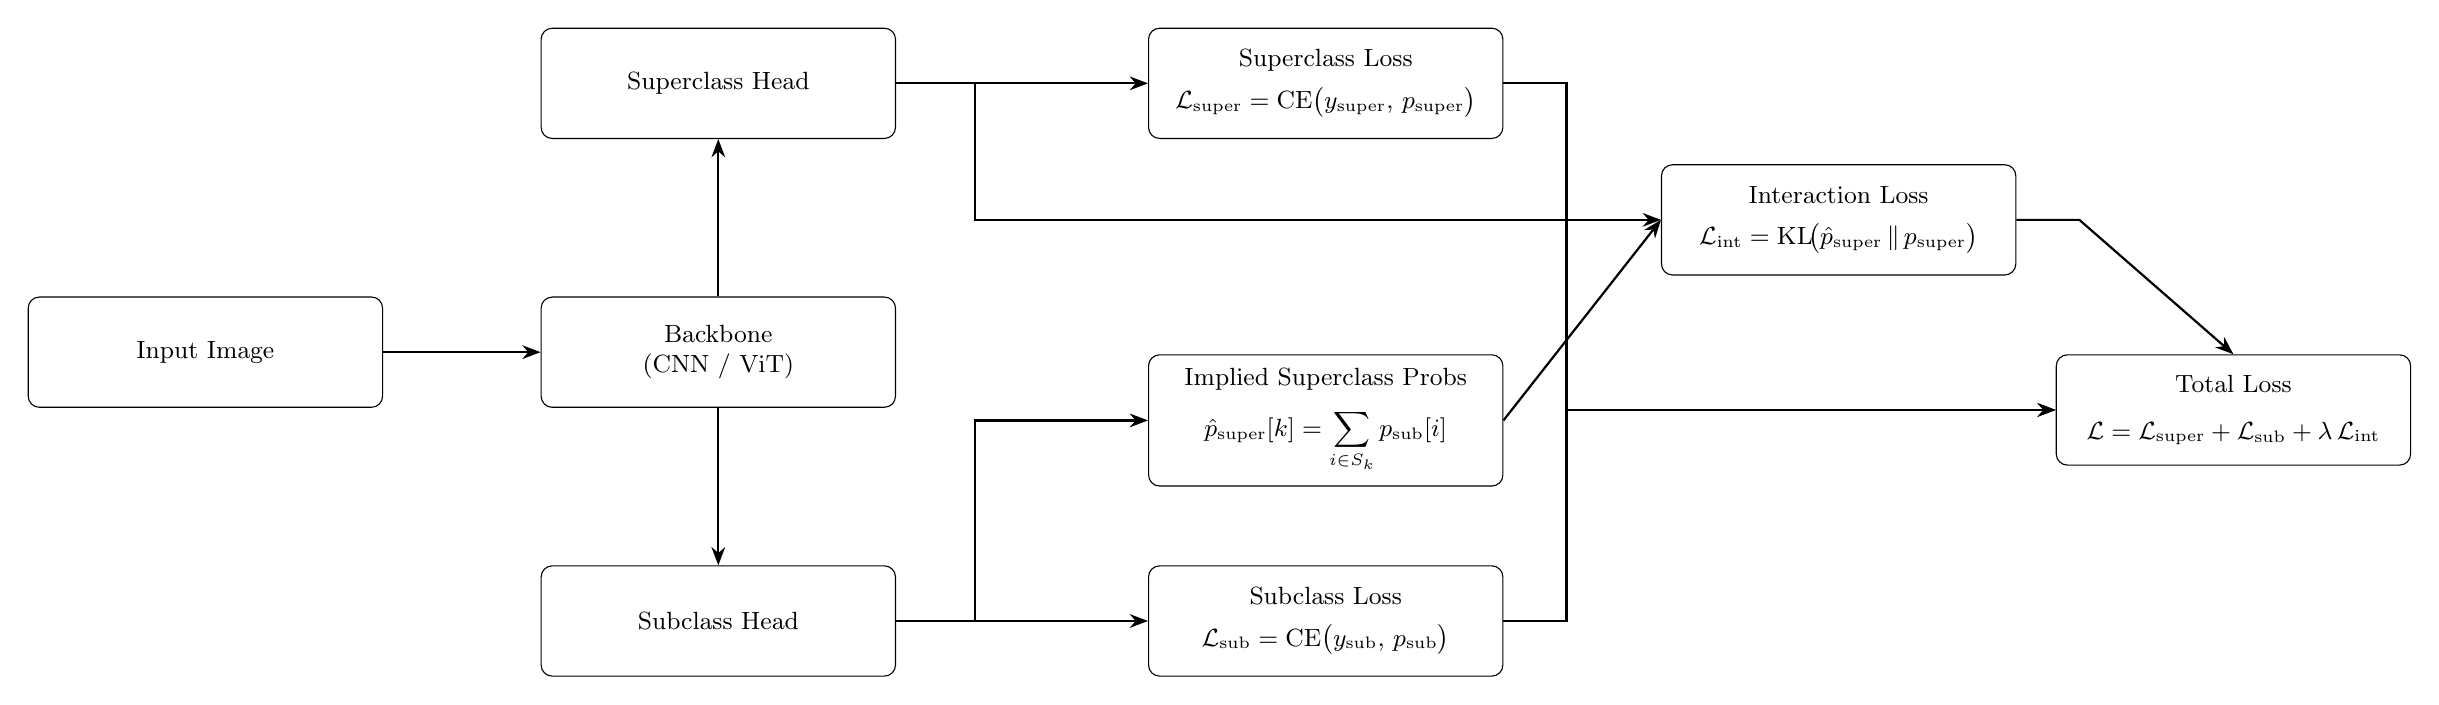
\begin{tikzpicture}[
								node distance = 2.5cm and 4.0cm,
								every node/.style={font=\small},
								box/.style={
										draw,
										rounded corners,
										align=center,
										minimum width=4.5cm,
										minimum height=1.4cm,
										inner sep=5pt
								},
								arrow/.style={-Stealth, thick}
						]

						% Main forward flow
						\node[box] (img) {Input Image};
						\node[box, right=2.0cm of img] (backbone) {Backbone\\(CNN / ViT)};

						% Heads (well separated vertically)
						\node[box, above=2.0cm of backbone] (superhead) {Superclass Head};
						\node[box, below=2.0cm of backbone] (subhead) {Subclass Head};

						% CE losses
						\node[box, right=3.2cm of superhead] (Lsuper) {Superclass Loss\\[4pt]
								$\mathcal{L}_{\text{super}}
						= \mathrm{CE}\big(y_{\text{super}},\, p_{\text{super}}\big)$};

						\node[box, right=3.2cm of subhead] (Lsub) {Subclass Loss\\[4pt]
								$\mathcal{L}_{\text{sub}}
						= \mathrm{CE}\big(y_{\text{sub}},\, p_{\text{sub}}\big)$};

						% Implied superclass probabilities from subclass head
						\node[box, above=1.0cm of Lsub] (qsuper) {Implied Superclass Probs\\[6pt]
								$\hat p_{\text{super}}[k]
						= \displaystyle \sum_{i \in S_k} p_{\text{sub}}[i]$};

						% Interaction (KL) loss: only uses implied and actual superclass probs
						\node[box, above right=1.0cm and 2cm of qsuper] (Lint) {Interaction Loss\\[4pt]
								$\mathcal{L}_{\text{int}}
						= \mathrm{KL}\!\big(\hat p_{\text{super}} \,\|\, p_{\text{super}}\big)$};

						% Total loss (sum of the three)
						\node[box, below right=1.0cm and 0.5cm of Lint] (Ltotal) {Total Loss\\[6pt]
								$\mathcal{L}
								= \mathcal{L}_{\text{super}}
								+ \mathcal{L}_{\text{sub}}
						+ \lambda\,\mathcal{L}_{\text{int}}$};

						% Main arrows
						\draw[arrow] (img) -- (backbone);

						\draw[arrow] (backbone) -- (superhead);
						\draw[arrow] (backbone) -- (subhead);

						\draw[arrow] (superhead) -- (Lsuper);
						\draw[arrow] (subhead) -- (Lsub);

						% From subclass head to implied superclass probs (only subclass → qsuper)
						\draw[arrow] (subhead.east) -- ++(1.0,0) |- (qsuper.west);

						% Interaction loss: only qsuper and superhead feed into it
						\draw[arrow] (qsuper.east) -- (Lint.west);
						\draw[arrow] (superhead.east) -- ++(1.0,0) |- (Lint.west);

						% Contributions to total loss: all three into Ltotal
						\draw[arrow] (Lsuper.east) -- ++(0.8,0) |- (Ltotal.west);
						\draw[arrow] (Lsub.east)   -- ++(0.8,0) |- (Ltotal.west);
						\draw[arrow] (Lint.east)   -- ++(0.8,0) -- (Ltotal.north);

				\end{tikzpicture}
		}
		\caption{Model architecture and loss computation.}
\end{figure}

\subsection{Interaction Loss / KL Divergence Calculations}

For each superclass $k$, with subclass set $S_k$:
\[
		\hat{p}_{\text{super}}[k]
  = \sum_{i \in S_k} p_{\text{sub}}[i].
\]

Then define interaction loss, e.g.:
\[
		\mathcal{L}_{\text{int}}
  = \mathrm{KL}\!\big(\hat{p}_{\text{super}} \,\|\, p_{\text{super}}\big).
\]

The Kullback--Leibler (KL) divergence between two distributions $P$ and $Q$ is:
\[
		\mathrm{KL}(P \,\|\, Q)
  = \sum_{k} P(k)\,\log \frac{P(k)}{Q(k)}.
\]

Equation below demonstrates math behind the KL divergence, which we used in Approach A.

\subsection{Approach B: Two independent models, separate for superclass and subclass}
Our second approach was adapting our architecture to have two separate ResNet-50 models,
one for superclass
and one for subclass. Each model has its own cross-entropy loss during training, and they
are independently
trained. At inference, their predictions are combined. The benefits of this approach are
that each model can
specialize for its particular classification task with little inference, the downside is
more parameters and
no consistency regularization.

\subsection{Approach C: Two independent models, separate for superclass and subclass
(cosine similarity head)}
Our third approach was to modify the subclass model to implement a cosine similarity head
instead of a linear feed-forward head.

\subsection{Evaluation}
The metrics used to evaluate model performance on unlabeled test data were: 1.
cross-entropy, 2. overall
accuracy, 3. seen accuracy and 4. unseen accuracy, all for both superclass and subclass.
We were limited to a
max of five leaderboard submissions.

\section{Experimental Settup}

Our hyperparameters were chosen as the following (for all models, unless denoted above):
Batch size of 64, 15
training epochs, learning rate of $10^{-4}$, weight decay of $10^{-4}$ for
generalization, and Adam as
optimizer. The hyperparameters used for the KL divergence term in Approach A was an alpha
value of 0.1 and a
Temperature value of 1.0. Lastly, We selected a $\tau_{\text{super}}$ of 0.99 and
$\tau_{\text{sub}}$ of 0.85
to threshold novel class predictions.

Below is a configuration table of our submissions, to illustrate differences in approaches.

\begin{table}[H]
		\centering
		\caption{Configuration table of submissions.}
		\label{tab:config}
		\begin{tabular}{@{}llllll@{}}
				\toprule
				Approach & Architecture & CIFAR novel super size & Backbone & Learning Rate & Head Type \\
				\midrule
				A & Two-heads  & 5000 & fine-tuned & .0001 & Linear\\
				B & Two models & 5000 & fine-tuned & .0001 & Linear\\
				C & Two models & 5000 & fine-tuned & .0001 & Super-Linear, Sub-Linear \\
				\bottomrule
		\end{tabular}
\end{table}

\section{Results}

Below table shows overall performance vs.\ baseline - the leaderboard test accuracy metrics:

\begin{table}[H]
		\centering
		\caption{Leaderboard test accuracy metrics.}
		\label{tab:results}
		\resizebox{\linewidth}{!}{%
				\begin{tabular}{@{}lcccccc@{}}
						\toprule
						Approach & Overall Super & Seen Super & Unseen Super & Overall Sub & Seen Sub & Unseen Sub \\
						\midrule
						A        & 83\% & 90\% & 63\% & 71\% & 84\% & 67\% \\
						B        & 85\% & 96\% & 57\% & 70\% & 83\% & 66\% \\
						C 		 & 90\%	&94\%	&79\%	&70\%	&75\%	&68\% \\
						\bottomrule
				\end{tabular}%
		}
\end{table}

\subsection{Analysis}
Overall, right from our initial Approach A and leaderboard submission we saw improved test accuracy
vs.\ baseline in all categories except ``Seen Super'' where we had 90\% accuracy for
Approach A vs.\ 99\%
baseline. This made sense to us, as there is an inherent tradeoff in maximizing seen
vs.\ unseen accuracies
when using a threshold to predict ``Novel'' classes. The tradeoff is that if you set a
lower threshold, say
90\% threshold instead of 99\% threshold as we did, we may have improved ``Seen''
accuracy at the expense of
``Novel'' accuracy since we would have reduced the rate of misclassifications labeled as
``Novel'' that were
actually ``Seen''. Since the goal was to improve the unseen accuracies vs.\ baseline, which we did
meaningfully for both Super and Sub, we are satisfied with these results. Thus, we kept
these thresholds
($\tau_{\text{sub}}$ and $\tau_{\text{super}}$) consistent for all of our approaches
accordingly. We will now
review the differences each approach was meant to isolate, one by one.

\subsection{Two-Heads vs. Two-Models performance}
Below demonstrates the key performance differences between these two approaches, with all
else held constant.
Notably, only the superclass performance diverged meaningfully, as subclass performance
was very similar. The
superclass performance on ``Seen'' superclasses improved for two-models, which is
intuitive as there was no
interaction between the two classifier heads (as the two-headed model faced). However,
the generalization
worsened as the superclass performance on ``Unseen'' superclasses decreased for
two-models, which makes sense
as the superclass model became relatively more overfit without the implicit
regularization of the shared
backbone \& KL-term.

\begin{figure}[H]
		\centering
		\includegraphics[width=0.95\linewidth]{fig_two_heads_vs_two_models.png}
		\caption{Performance delta between Two-Heads and Two-Models.}
		\label{fig:two_heads_vs_two_models}
\end{figure}

\subsection{$5{,}000$ vs. $1{,}000$ CIFAR-100 ``Novel'' Superclass Images Added performance}
Interestingly, reducing the number of ``Novel'' class superclass images added to the
training data only
affected the superclass accuracy performance very little. We suppose this is from
$1{,}000$ CIFAR-100 being
of sufficient size (relative to $\sim 6{,}600$ original training images) for the model to
learn the patterns
of the subspace of images that do not represent a bird, dog, or reptile, such that
additional random examples
from this complement space do not notably improve the accuracy.

However, for subclass accuracy, we observe meaningful differences. Notably, when we
reduce the amount of
images added (labeled as Novel superclass), we worsen performance on seen subclasses, but
meaningfully
improve performance on unseen subclasses. Given that this was tested on the two-model
architecture, where the
only training data with ``Novel'' subclasses would be images that are not birds, dogs and
reptiles, the most
plausible explanation is that we were ``teaching'' the model that novel subclasses come
from a distribution
beyond the superclasses of the training data. Therefore, when we relax this constraint
(less images added),
we reduce the ``overfitting'' to that constrained case of subclasses out of training
distribution, and thus
we improve on generalization of subclass accuracy for unseen subclasses in test data. We
expect the model
with less images added is more ``naive'' to the distribution of natural images.

\begin{figure}[H]
		\centering
		\includegraphics[width=0.95\linewidth]{fig_5000_vs_1000.png}
		\caption{Performance delta between 5{,}000 and 1{,}000 superclass images added.}
		\label{fig:5000_vs_1000}
\end{figure}

\subsection{Amount of Fine-Tuning for Transfer Learning (Full fine-tuning vs.\ Fixed backbone)}
Here we changed from full fine-tuning (with a learning rate of 0.0001) to fixing the
ResNet50 backbone and
only fine-tuning a single linear layer on top (with a learning rate of 0.01). This led to our worst
performance, with the performance on subclasses meaningfully worse across the board
vs.\ any of our other
approaches (for overall, seen, and super). This makes sense as we likely had too high a
learning rate to
learn nuances between dogs/reptiles/birds well. The results for superclass accuracy were
more interesting, as
the seen superclass performance was worse, but the unseen superclass performance the best
out of all of our
approaches. We think this is because only the single linear layer was tuned on the
superclass model, so it
was able to specialize in identifying a ``Novel'' superclass vs.\ having that signal distorted when
propagated across the full backbone (as in our other approaches).

\begin{figure}[H]
		\centering
		\includegraphics[width=0.95\linewidth]{fig_finetune_vs_frozen.png}
		\caption{Performance delta between full fine-tuning and fixed backbone.}
		\label{fig:finetune_vs_frozen}
\end{figure}

\section{Discussion and Limitations}

Our best model demonstrates (Approach B) demonstrates good performance on seen super and
subclasses, and
$\sim 60\%$ performance of catching novel super and subclasses in test data. We note that
at the time of
writing, this model's performance seems to exceed that of most other ResNet-based
architectures on the
leaderboard, though surpassed by vision transformer-based architectures.

Limitations exist in our use of CIFAR and ``pseudo-novel'' subclass holdout as proxies
for calibrating our
thresholds for inference of ``Novel'' superclass and subclass respectively. CIFAR-100 served as an
approximation for showing the model ``out of distribution'' superclass data, but did not
necessarily include
ambiguous data on the margin. Neither did our ``pseudo-novel'' technique necessarily
teach our model to learn
the full subspace of dog breeds (or reptiles/birds). Since there is a natural confidence
overlap between seen
and novel, we always faced the tradeoff in determining at what discrete point the
boundary should lie.

We initially expected a single model with two heads and KL divergence term would be
higher performing, due to
its seemingly greater sophistication and unifying approach. We were surprised to learn,
however, that two
models trained separately perform better on our test data. Additionally, our initial
instinct was that
freezing the transfer learning backbone and only fine-tuning a layer on top would be
superior, but apart from
the unseen superclass evaluation metric, it was not. Lastly, it was also very surprising
that reducing the
amount of CIFAR superclass data affected the subclass performance much more noticeably
than the superclass
performance, though now we better appreciate the inherent complexity and sensitivity to
change of neural networks.

\section{Conclusion \& Future Work}

We experimented with various strategies to maximize performance on this transfer-learning image
classification task. The approaches pursued were changing architecture (single model with
		two heads + KL
divergence term vs.\ two models), changing number of extra images added to training data ($5{,}000$
vs.\ $1{,}000$), and changing the amount of fine-tuning (full fine-tuning vs.\ fixed
backbone). Our best
model was using two separate models, with $5{,}000$ novel superclass images added, and
performing full fine-tuning.

Given further time and resources, we would have spent more time curating out of
distribution datasets to add
to the training data (in particular, images from novel subclasses from the given
		superclasses, as in new dog
breeds, reptiles, and birds). We would have explored implementing more advanced and
modern architecture such
as Vision-Transformers.

\section{Appendix \& Links}

The code for our experiments can be found at:
\url{https://github.com/akseldkw07/NNDL-Project/tree/main}.

The notebook used for training can be found within the repository at
\url{https://github.com/akseldkw07/NNDL-Project/blob/main/NNDL_PROJECT_FINAL/NNDL_Project_Notebook_Live_Submit.ipynb}

\clearpage
\begin{thebibliography}{99}

		\bibitem{Donahue2014}
		\textbf{J.~Donahue}, \textbf{Y.~Jia}, \textbf{O.~Vinyals}, \textbf{J.~Hoffman}, \textbf{N.~Zhang},
		\textbf{E.~Tzeng}, and \textbf{T.~Darrell}.
		DeCAF: A Deep Convolutional Activation Feature for Generic Visual Recognition.
		In \emph{Proceedings of the 31st ICML}, 2014.

		\bibitem{Krizhevsky2012}
		\textbf{A.~Krizhevsky}, \textbf{I.~Sutskever}, and \textbf{G.~E.~Hinton}.
		ImageNet Classification with Deep Convolutional Neural Networks.
		In \emph{Advances in Neural Information Processing Systems (NeurIPS)}, 2012.

		\bibitem{Caruana1997}
		\textbf{R.~Caruana}.
		Multitask Learning.
		\emph{Machine Learning}, 28(1):41--75, 1997.

		\bibitem{Hinton2015}
		\textbf{G.~Hinton}, \textbf{O.~Vinyals}, and \textbf{J.~Dean}.
		Distilling the Knowledge in a Neural Network.
		In \emph{NIPS Deep Learning and Representation Learning Workshop}, 2015.

		\bibitem{He2016}
		\textbf{K.~He}, \textbf{X.~Zhang}, \textbf{S.~Ren}, and \textbf{J.~Sun}.
		Deep Residual Learning for Image Recognition.
		In \emph{CVPR}, 2016.

		\bibitem{Yosinski2014}
		\textbf{J.~Yosinski}, \textbf{J.~Clune}, \textbf{Y.~Bengio}, and \textbf{H.~Lipson}.
		How Transferable Are Features in Deep Neural Networks?
		In \emph{NeurIPS}, 2014.

		\bibitem{PanYang2010}
		\textbf{S.~J.~Pan} and \textbf{Q.~Yang}.
		A Survey on Transfer Learning.
		\emph{IEEE Transactions on Knowledge and Data Engineering}, 22(10):1345--1359, 2010.

		\bibitem{BendaleBoult2016}
		\textbf{A.~Bendale} and \textbf{T.~E.~Boult}.
		Towards Open Set Deep Networks.
		In \emph{CVPR}, 2016.

		\bibitem{HendrycksGimpel2017}
		\textbf{D.~Hendrycks} and \textbf{K.~Gimpel}.
		A Baseline for Detecting Misclassified and Out-of-Distribution Examples in Neural Networks.
		In \emph{ICLR}, 2017.

		\bibitem{Goyal2017}
		\textbf{P.~Goyal}, \textbf{P.~Doll\'ar}, \textbf{R.~Girshick}, \textbf{P.~Noordhuis},
		\textbf{L.~Wesolowski}, \textbf{A.~Kyrola}, \textbf{A.~Tulloch}, \textbf{Y.~Jia}, and
		\textbf{K.~He}.
		Accurate, Large Minibatch SGD: Training ImageNet in 1 Hour.
		\emph{arXiv:1706.02677}, 2017.

\end{thebibliography}

\end{document}
